\documentclass[12pt]{beamer}
\usepackage{../Estilos/BeamerMAF}
\usepackage{../Estilos/ColoresLatex}
\input{../Preambulos/preambulo_Beamer_Cambridge_beaver}

\date{}

\title{\large{La delta de Dirac}}
\subtitle{Tema 2 - Primeras técnicas de solución}
\author{M. en C. Gustavo Contreras Mayén}

\resetcounteronoverlays{saveenumi}

\begin{document}
\maketitle
\fontsize{14}{14}\selectfont
\spanishdecimal{.}

\section*{Contenido}
\frame{\tableofcontents[currentsection, hideallsubsections]}

\section{Concepto inicial}
\frame[allowframebreaks]{\tableofcontents[currentsection, hideothersubsections]}
\subsection{Introducción}

\begin{frame}
\frametitle{Referencia inicial}
En física a menudo nos encontramos con fenómenos donde se involucra el concepto de un pulso de duración \enquote{infinitamente corto}.
\end{frame}

\begin{frame}
\frametitle{Ejemplo de pulso corto}
Por ejemplo, en su curso de Mecánica Clásica se revisó el concepto de una magnitud física llamada \textocolor{red}{impulso}, \pause la cual se introduce cuando se cambia el estado de movimiento de un cuerpo al aplicarle un \enquote{golpe repentino}.
\\
\bigskip
\pause
El impulso se denota comúnmente con la letra $I$.
\end{frame}

\begin{frame}
\frametitle{Ejemplo de pulso corto}
Tomemos como ejemplo del fútbol, con un penalty, \pause en este caso tenemos inicialmente al balón en reposo, \pause la intención es meter la pelota en la portería contraria.
\end{frame}

\begin{frame}
\frametitle{Ejemplo de pulso corto}
Después de patear el balón, éste adquiere un momento que es igual al impulso asociado a la patada misma.
\\
\bigskip
\pause
Analíticamente esta afirmación se escribe como:
\pause
\begin{align*}
m \, v = I = \scaleint{6ex}_{\bs t_{0}}^{t_{0} + \tau} F (t) \dd{t}
\end{align*}
donde $F (t)$ es la fuerza y $\tau$ la duración del impacto sobre la pelota (técnicamente de la acción de la fuerza sobre el balón).
\end{frame}

\begin{frame}
\frametitle{Analizando el ejemplo}
El término \textocolor{cadmiumgreen}{repentino} implica que $\tau$ se considera infinitamente pequeño \pause y por tanto, que el cambio en el momento ocurre instantáneamente.
\end{frame}

\begin{frame}
\frametitle{Ejemplo de pulso corto}
Sin embargo, dado que el cambio en el momento es un número finito, \pause se sigue que la magnitud de la fuerza $F (t)$ debió haber sido infinita durante el golpe al balón y cero en cualquier otro momento.
\end{frame}

\begin{frame}
\frametitle{Representación matemática}
Este tipo de descripciones no se puede formular apropiadamente con los conceptos matemáticos que conocemos, más aún, la descripción tampoco es rigurosa desde un punto de vista físico.
\end{frame}

\begin{frame}
\frametitle{Gráfica de pulso corto}
\begin{figure}[H]
    \centering
    \includegraphics[scale=0.85]{Imagenes/ejemplo_delta_Dirac_01.pdf}
    \caption{Representación del pico para la función.}
    \label{fig:figura_delta_Dirac_01}
\end{figure}
\end{frame}

\begin{frame}
\frametitle{Revisando la gráfica}
En realidad, la gráfica de la fuerza es una curva muy \enquote{\textocolor{ao}{picuda}}: muy estrecha y muy alta, como se aprecia en la figura (\ref{fig:figura_delta_Dirac_01}) \pause y satisface la propiedad que el área bajo la curva es igual a $I$.
\end{frame}

\begin{frame}
\frametitle{El caso en la física}
En la gran mayoría de los problemas físicos, la forma exacta de la gráfica no se conoce, \pause sin embargo, en lo correspondiente a los efectos físicos observables asociados con tal función, usualmente esta falta de información no importa.
\end{frame}

\begin{frame}
\frametitle{Valor del impulso}
Lo que tiene significado es la integral de la fuerza, esto es, el valor del impulso:
\pause
\begin{align*}
I = \scaleint{6ex}_{\bs t_{0}}^{t_{0} + \tau } F (t) \dd{t}
\end{align*}
\end{frame}

\begin{frame}
\frametitle{De las funciones puntiagudas}
Las funciones puntiagudas son comunes en cualquier área de la física, \pause por ejemplo: una fuerza concentrada sobre una barra, es una distribución puntiaguda de la carga, \pause veamos las figuras (\ref{fig:figura_delta_Dirac_02}) y (\ref{fig:figura_delta_Dirac_03}). 
\end{frame}

\begin{frame}
\frametitle{Función puntiaguda ideal}
\begin{figure}[H]
    \centering
    \includegraphics[scale=1]{Imagenes/ejemplo_delta_Dirac_02.pdf}
    \caption{Representación de una fuerza aplicada de manera ideal.}
    \label{fig:figura_delta_Dirac_02}
\end{figure}
\end{frame}

\begin{frame}
\frametitle{Función puntiaguada real}
\begin{figure}[H]
    \centering
    \includegraphics[scale=1]{Imagenes/ejemplo_delta_Dirac_03.pdf}
    \caption{Representación de una fuerza aplicada de manera real.}
    \label{fig:figura_delta_Dirac_03}
\end{figure}
\end{frame}

\begin{frame}
\frametitle{Otras funciones puntiagudas}
En los circuitos eléctricos, las corrientes \textocolor{cadetblue}{puntiagudas} de una duración extremadamente corta, \pause se presentan cuando se conecta el interruptor, como en el caso de la redistribución de carga entre dos condensadores, como se ve en la figura (\ref{fig_figura_delta_Dirac_04}).
\end{frame}

\begin{frame}
\frametitle{Función puntiaguda en un circuito eléctrico}
\begin{figure}[H]
    \centering
    \includegraphics[scale=1]{Imagenes/ejemplo_circuito_delta.pdf}
    \caption{Circuito eléctrico antes de cerrar el interruptor.}
    \label{fig_figura_delta_Dirac_04}
\end{figure}
\end{frame}

% \section{Teoría de distribuciones}
% \frame[allowframebreaks]{\tableofcontents[currentsection, hideothersubsections]}
% \subsection{Referencia breve}

% \begin{frame}
% \frametitle{Antecedente histórico}
% Las ideas que nos permitieron desarrollar el concepto de la delta de Dirac previamente, se pueden sistematizar en lo que se conoce como \textocolor{carmine}{la teoría de distribuciones o funciones generalizadas}.
% \end{frame}

% \begin{frame}
% \frametitle{Autor principal}
% Las funciones generalizadas fueron introducidas en 1935 por el matemático ruso, Sergei Lvóvich Sóbolev (1908 - 1989).
% \begin{figure}
%     \centering
%     \includegraphics[scale=0.25]{Imagenes/Serguei_Sobolev.jpg}
% \end{figure}
% \end{frame}

% \begin{frame}
% \frametitle{Continuando la teoría}
% De manera independientemente a finales de la década de 1940, el matemático francés, Laurent Schwartz (1915 - 2002) formalizó la teoría de distribuciones, \pause lo que le valió la Medalla Fields en 1950.
% \end{frame}
% \begin{frame}
% \frametitle{Premio no recibido}
% Que no recibió durante la entrega, ya que se le negó la visa para ingresar a los Estados Unidos.
% \begin{figure}
%     \centering
%     \includegraphics[scale=0.35]{Imagenes/Laurent_Schwartz.jpg}
% \end{figure}
% \end{frame}

% \begin{frame}
% \frametitle{Intención de la teoría}
% Como el nombre lo sugiere, la teoría tiene como objetivo  \textocolor{cobalt}{extender la definición de una función}, \pause de manera tal que conceptos como el de la delta de Dirac $\delta (x)$ cuenten con una base matemática firme.
% \end{frame}

% \begin{frame}
% \frametitle{Intención de la teoría}
% En particular la teoría permite extender el concepto de derivada a todas las funciones localmente integrables y a entes aún más generales.
% \end{frame}

% \begin{frame}
% \frametitle{Integrales de estudio}
% Existen varias formas de presentar la teoría de distribuciones, se dará una breve introducción utilizando las integrales de secuencias de funciones del tipo:
% \pause
% \begin{equation}
% \scaleint{6ex} f_{n} (x) \, g (x) \dd{x} \hspace{1cm} n = 1, 2, 3 , \ldots
% \label{eq:ecuacion_1_99}
% \end{equation}
% \end{frame}

% \begin{frame}
% \frametitle{Conceptos importantes}
% Para ello es necesario introducir tres conceptos:
% \pause
% \setbeamercolor{item projected}{bg=bananayellow,fg=ao}
% \setbeamertemplate{enumerate items}{%
% \usebeamercolor[bg]{item projected}%
% \raisebox{1.5pt}{\colorbox{bg}{\color{fg}\footnotesize\insertenumlabel}}%
% }
% \begin{enumerate}[<+->]
% \item El concepto de función de prueba.
% \item El concepto de función admisible.
% \item El concepto de convergencia débil.
% \end{enumerate}
% \end{frame}

% \begin{frame}
% \frametitle{Secuencia de funciones}
% Hemos visto que una secuencia de funciones $f_{n} (x)$ tal como la secuencia delta de funciones, definida en \ref{secuencias_delta}, \pause nos lleva al concepto matemático de \enquote{función} delta, si la secuencia de integrales converge para funciones apropiadas $g (x)$.
% \end{frame}

% \begin{frame}
% \frametitle{Pregunta interesante}
% Pero \textocolor{carmine}{¿qué quiere decir que sean apropiadas?}
% \pause
% Si queremos definir conceptos tales como las \textbf{derivadas de la función delta}, entonces las funciones $g (x)$ deben ser diferenciables.
% \end{frame}

% \begin{frame}
% \frametitle{Derivadas de las funciones}
% Para definir las derivadas también hemos visto que al integrar por partes, para que las derivadas totales no contribuyan, es necesario que la función $g (x)$ tenga un comportamiento apropiado en infinito.
% \end{frame}

% \begin{frame}
% \frametitle{Las funciones apropiadas}
% Definimos entonces las funciones $g (x)$ como:
% \pause
% Decimos que las función $g (x)$ en la ec. (\ref{eq:ecuacion_1_99}), es una \textocolor{darkgreen}{función de prueba}, si es infinitamente diferenciable (clase $C^{\infty}$) y es idénticamente cero fuera de algún intervalo $(a, b)$ (en general este intervalo es diferente para funciones $g (x)$ diferentes).
% \end{frame}

% \begin{frame}
% \frametitle{Las funciones de prueba}
% El nombre de funciones de prueba es adecuado, dado que por ejemplo, \textocolor{alizarin}{la propiedad de filtro} de las secuencias delta, se prueba sobre estas funciones.
% \end{frame}

% \begin{frame}
% \frametitle{Requerimiento de otras funciones}
% Habiendo definido las funciones de prueba, podemos ahora definir las \textocolor{amethyst}{funciones admisibles} (de las cuales seleccionaremos las funciones $f_{n}( x)$) y la \textocolor{americanrose}{convergencia débil}.
% \end{frame}

% \begin{frame}
% \frametitle{Funciones admisibles}
% Decimos que las funciones $f_{n} (x)$ en la ec. (\ref{eq:ecuacion_1_99}) son \textocolor{antiquefuchsia}{funciones admisibles}, si son infinitamente diferenciables.
% \\
% \bigskip
% \pause
% Su comportamiento en infinito puede ser arbitrario.
% \end{frame}

% \begin{frame}
% \frametitle{Convergencia débil}
% Consideremos una secuencia de funciones admisibles $f_{n} (x)$ con $n = 1, 2, 3, \ldots$
% \\
% \bigskip
% \pause
% Decimos que esta secuencia es débilmente convergente si el límite:
% \pause
% \begin{equation}
% \lim_{n \to \infty} \scaleint{6ex}_{\bs -\infty}^{\infty} f_{n}(x) \:  g (x) \, \dd{x}
% \label{eq:ecuacion_1_100}
% \end{equation}
% existe para todas las funciones de prueba $g (x)$.
% \end{frame}

% \begin{frame}
% \frametitle{Secuencias débilmente convergentes}
% Una secuencia débilmente convergente puede o no puede converger en alguno de los sentidos de convergencia usual, como convergencia puntual.
% \end{frame}

% \begin{frame}
% \frametitle{Concepto de distribución}
% Podemos presentar ahora una definición rigurosa de una distribución de la siguiente manera:
% \pause
% Una \textocolor{auburn}{distribución} $\varphi (x)$ es un concepto matemático asociado con una secuencia débilmente convergente de funciones admisibles para la cual la integral simbólica:
% \pause
% \begin{equation}
% \scaleint{6ex}_{\bs -\infty}^{\infty} \phi (x) \:  g (x) \, \dd{x}
% \label{eq:ecuacion_1_101}
% \end{equation}
% \end{frame}

% \begin{frame}
% \frametitle{Significado de la distribución}
% Tiene un significado preciso, por medio de la prescripción:
% \pause
% \begin{equation}
% \scaleint{6ex}_{\bs -\infty}^{\infty} \phi (x) \: g (x) \, \dd{x} = \lim_{n \to \infty} f_{n} (x) \: g (x) \, \dd{x}
% \label{eq:ecuacion_1_102}
% \end{equation}
% \end{frame}

\section{La delta de Dirac}
\frame[allowframebreaks]{\tableofcontents[currentsection, hideothersubsections]}
\subsection{Definición}

\begin{frame}
\frametitle{Expresando la delta de Dirac}
Informalmente la delta de Dirac es una \enquote{\textocolor{blue-violet}{función}} que representa un pico infinitamente agudo expresado simbólicamente por:
\pause
\begin{equation}
\delta (x) = \begin{cases}
0 & x \neq 0 \\
\infty & x = 0
\end{cases}
\label{eq:ecuacion_delta_01}
\end{equation}
\end{frame}

\begin{frame}
\frametitle{Integral normalizada}
Pero tal que la integral de $\delta (x)$ está normalizada a la unidad:
\pause
\begin{equation}
\scaleint{6ex}_{\bs -\infty}^{\infty} \delta (x) \: \dd{x} = 1 
\label{eq:ecuacion_delta_02}
\end{equation}
\end{frame}

\subsection{Propiedad de filtro}

\begin{frame}
\frametitle{Propiedades de la $\delta (x)$}
La delta de Dirac satisface la siguiente propiedad:
\pause
\begin{equation}
\scaleint{6ex}_{\bs -\infty}^{\infty} \delta (x) \: f (x) \: \dd{x} = f (0)
\label{eq:ecuacion_delta_03}
\end{equation}
donde $f (x)$ es una función continua.
\end{frame}

\begin{frame}
\frametitle{Resolviendo la integral}
Esta integral puede ser \enquote{\textocolor{red}{evaluada}} utilizando siguiente argumento: \pause
\setbeamercolor{item projected}{bg=bole,fg=white}
\setbeamertemplate{enumerate items}{%
\usebeamercolor[bg]{item projected}%
\raisebox{1.5pt}{\colorbox{bg}{\color{fg}\footnotesize\insertenumlabel}}%
}
\begin{enumerate}[<+->]
\item Dado que $\delta (x) = 0$ para $x \neq 0$.
\item Podemos cambiar los límites de integración en la ecuación (\ref{eq:ecuacion_delta_03}) a $- \epsilon$ y $+ \epsilon$, donde $\epsilon$ es un número positivo infinitesimal.
\seti
\end{enumerate}
\end{frame}

\begin{frame}
\frametitle{Resolviendo la integral}
\setbeamercolor{item projected}{bg=bole,fg=white}
\setbeamertemplate{enumerate items}{%
\usebeamercolor[bg]{item projected}%
\raisebox{1.5pt}{\colorbox{bg}{\color{fg}\footnotesize\insertenumlabel}}%
}
\begin{enumerate}[<+->]
\conti
\item Más aún, dado que $f (x)$ es continua en $x = 0$, sus valores dentro del intervalo $( - \epsilon, + \epsilon)$ no diferirán mucho de $f (0)$ y podemos hacer la siguiente aproximación:
\begin{eqnarray*}
\begin{aligned}
\scaleint{6ex}_{\bs -\infty}^{\infty} \delta (x) \: f (x) \: \dd{x} &= \scaleint{6ex}_{\bs -\epsilon}^{\epsilon} \delta (x) \: f (x) \: \dd{x} \\[0.5em] \pause
&\approx f (0) \scaleint{6ex}_{\bs -\infty}^{\infty} \delta (x) \: \dd{x}
\end{aligned}
\end{eqnarray*}
Esta aproximación mejora cuando $\epsilon \to 0$.
\end{enumerate}
\end{frame}

\begin{frame}
\frametitle{Consideración importante}
Pero:
\pause
\begin{align*}
\scaleint{6ex}_{\bs -\epsilon}^{+\epsilon} \delta (x) \: \dd{x} = 1
\end{align*}
para todos los valores de $\epsilon$, por que $\delta (x) = 0$ para $x \neq 0$ y $\delta (x)$ está normalizada.
\end{frame}

\begin{frame}
\frametitle{Tomando el límite}
Así en el límite $\epsilon \to 0$, se tiene:
\pause
\begin{align*}
\scaleint{6ex}_{\bs -\infty}^{\infty} \delta (x) \: f (x) \: \dd{x} = f (0)
\end{align*}
\textbf{Nota: } Los límites $-\infty$ y $+\infty$ se pueden reemplazar por cualesquiera números $a$ y $b$, tales que $a < 0 < b$.
\end{frame}

\begin{frame}
\frametitle{Propiedad de filtro}
Esta integral se le conoce también como \textocolor{bostonuniversityred}{propiedad de filtro} de la función delta, \pause ya que $\delta (x)$ actúa como un filtro, seleccionando de todos los posibles valores de $f (x)$ su valor en el punto $x = 0$.
\end{frame}

\subsection{Secuencias delta}\label{secuencias_delta}

\begin{frame}
\frametitle{Haciendo la referencia correcta}
La afirmación de que la función $\delta (x)$ está dada por la expresión (\ref{eq:ecuacion_delta_01}) \textit{\textocolor{brown(web)}{o es una afirmación apropiada y no se puede utilizar para definir una función}}, mucho menos para una función integrable.
\end{frame}

\begin{frame}
\frametitle{Referencia alterna}
Una posible definición alterna, podría ser el definir la función $\delta (x)$ como la función que satisface la propiedad de filtro (\ref{eq:ecuacion_delta_03}):
\pause
\begin{align*}
\scaleint{6ex}_{\bs -\infty}^{+ \infty} \delta (x) \: f (x) \: \dd{x} = f (0)
\end{align*}
para toda función continua $f (x)$. 
\end{frame}

\begin{frame}
\frametitle{Complicación matemática}
Sin embargo es posible demostrar que no existe ninguna función con esa propiedad.
\\
\bigskip
\pause
Por lo que:
\pause
\begin{center}
\textit{¡¡la función delta no es una función en el sentido matemático usual!!}
\end{center}
\end{frame}

\begin{frame}
\frametitle{Respondiendo al problema}
¿Qué se hace entonces? \pause ¿Dirac nos engañó con su propuesta?
\\
\bigskip
\pause
Lo que sucede es que existen secuencias de funciones de pico pronunciado, las cuales en el límite en que el pico es infinitamente delgado e infinitamente alto, satisfacen la propiedad de filtro.
\end{frame}

\begin{frame}
\frametitle{Proponiendo una secuencia}
La siguiente puede ser una secuencia $\phi_{n} (x)$ con $n = 1, 2, 3, \ldots$, tal que:
\pause
\begin{align*}
\lim_{n \to \infty} \scaleint{6ex}_{\bs -\infty}^{+ \infty} \phi_{n} (x) \: f (x) \dd{x} =  f (0)
\end{align*}
\end{frame}

\begin{frame}
\frametitle{Definiendo la secuencia delta}
Llamamos secuencias delta $\delta_{n} (x)$ a una secuencia de funciones de pico pronunciado, que satisfacen:
\pause
\begin{align*}
\lim_{n \to \infty} \scaleint{6ex}_{\bs -\infty}^{+ \infty} \phi_{n} (x) \: f (x) \: \dd{x} =  f (0)
\end{align*}
\end{frame}

\begin{frame}
\frametitle{Ejemplo de una secuencia}
La secuencia de funciones:
\pause
\begin{equation}
\phi_{n} (x) = \begin{cases}
0 & x < - \dfrac{1}{2 \, n} \\
n & - \dfrac{1}{2 \, n} < x < \dfrac{1}{2 \, n} \\
0 & 0 >  \dfrac{1}{2 \, n}
\end{cases}
\hspace{1cm} n = 1, 2, 3, \ldots
\label{eq:ecuacion_delta_04}
\end{equation}
es una secuencia delta.
\end{frame}

\begin{frame}[plain]
%\frametitle{Graficando la secuencia}
\begin{figure}[H]
    \centering
    \includegraphics[scale=0.5]{Imagenes/plot_secuencia_delta.pdf}
    \caption{Secuencia delta para valores de $n = 1, 2, \ldots, 10$. El área debajo de la curva para cada $\phi_{n}$ siempre es $1$.}
    \label{fig:secuncia_delta_01}
\end{figure}
\end{frame}

\begin{frame}
\frametitle{Demostración}
Para verificar esta afirmación consideremos la integral:
\pause
%Apuntes FETI página 46
\begin{align*}
\scaleint{6ex}_{\bs -\infty}^{\infty} \phi_{n} (x) \: f (x) \dd{x}
\end{align*}
para cualquier función continua arbitraria $f (x)$.
\end{frame}

\begin{frame}
\frametitle{Demostración}
De la expresión (\ref{eq:ecuacion_delta_04}) para la secuencia delta se tiene:
\pause
\begin{eqnarray*}
\scaleint{6ex}_{\bs -\infty}^{+ \infty} \phi_{n} (x) \: f (x) \dd{x} &=  \pause \scaleint{6ex}_{\bs -\frac{1}{2 \, n}}^{\frac{1}{2 \, n}} n \: f (x) \: \dd{x} = \\[0.5em] \pause
&= n \scaleint{6ex}_{\bs -\frac{1}{2 \, n}}^{\frac{1}{2 \, n}} f (x) \:  \dd{x}
\end{eqnarray*}
\end{frame}

\begin{frame}
\frametitle{Apoyo del cálculo}
Utilizando el teorema del valor medio para integrales, podemos deducir que:
\pause
\begin{eqnarray*}
\begin{aligned}
n \, \scaleint{6ex}_{\bs -\frac{1}{2 \, n}}^{\frac{1}{2 \, n}} f (x) \dd{x} \pause &= n \: \dfrac{1}{n} f (\xi) = \\[0.5em] \pause
&= f (\xi), \hspace{1cm} - \dfrac{1}{2 \, n} \leq \xi \leq \dfrac{1}{2 \, n}
\end{aligned}
\end{eqnarray*}
En el límite cuando $n \to \infty$, $\xi \to 0$.
\end{frame}

\begin{frame}
\frametitle{Usando la continuidad de la función}
De la continuidad de la función $f (x)$ se sigue que $f (\xi) \to f (0)$, obteniendo así el resultado:
\pause
\begin{align*}
\lim_{n \to \infty} \scaleint{6ex}_{\bs -\infty}^{+ \infty} \: \phi_{n} (x) \: f (x) \: \dd{x} = f (0)
\end{align*}
lo que nos dice que la secuencia (\ref{eq:ecuacion_delta_04}), es una secuencia delta. \pause  Nótese que la secuencia delta (\ref{eq:ecuacion_delta_04}) no es derivable en el punto $x = 0$.
\end{frame}

\begin{frame}
\frametitle{Secuencias atractivas y de utilidad}
Para muchos propósitos es deseable construir secuencias delta de funciones que sean continuas y diferenciables.
\\
\bigskip
\pause 
Por ejemplo, en las figuras (\ref{fig:plot_secuencia_01}), (\ref{fig:plot_secuencia_02}) y (\ref{fig:plot_secuencia_03}) podemos apreciar algunas secuencias delta con estas características:
\end{frame}

\begin{frame}[plain]
\frametitle{Una secuencia delta}
\begin{figure}[H]
    \centering
    \includegraphics[scale=0.7]{Imagenes/secuencia_delta_01.pdf}
    \caption{Secuencia para $\phi_{n}$ con $n=1,2,3$}
    \label{fig:plot_secuencia_01}
\end{figure}
\end{frame}

\begin{frame}
\frametitle{Otra secuencia delta}
\begin{figure}[H]
    \centering
    \includegraphics[scale=0.7]{Imagenes/secuencia_delta_02.pdf}
    \caption{Secuencia para $\phi_{n}$ con una función exponencial.}
    \label{fig:plot_secuencia_02}
\end{figure}
\end{frame}

\begin{frame}
\frametitle{Una secuencia delta más}
\begin{figure}[H]
    \centering
    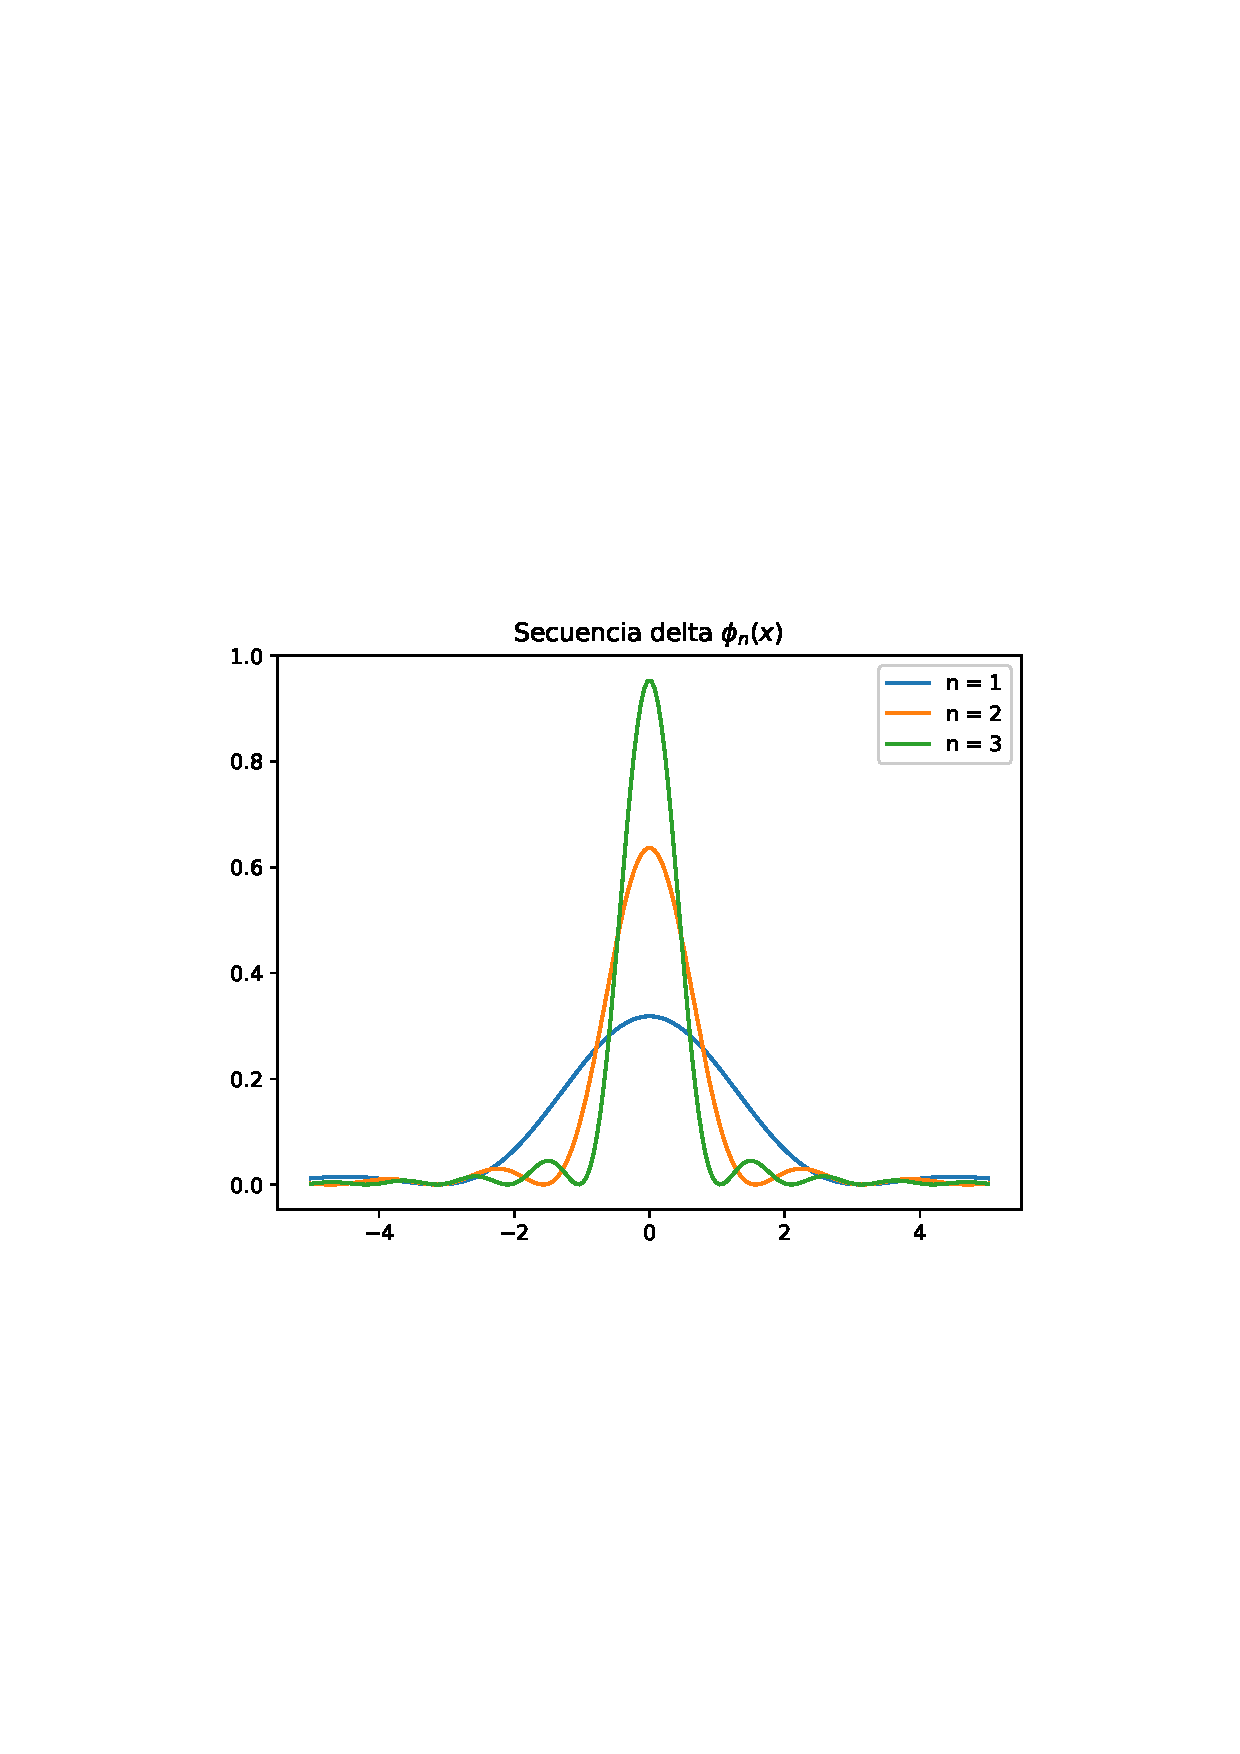
\includegraphics[scale=0.65]{Imagenes/secuencia_delta_03.pdf}
    \caption{Secuencia para $\phi_{n}$ con una función $\sin^{2}(x)/x$}
    \label{fig:plot_secuencia_03}
\end{figure}
\end{frame}

\begin{frame}
\frametitle{Consideración relevante}
Tomemos en cuenta que no es correcto expresar que éstas secuencias convergen a la función delta: \pause los límites de esas secuencias \textocolor{burgundy}{no existen}, de acuerdo a las definiciones conocidas de convergencia.
\end{frame}

\begin{frame}
\frametitle{Secuencias normalizadas}
Todas estas funciones están normalizadas a la unidad:
\pause
\begin{equation}
\lim_{n \to \infty} \scaleint{6ex}_{\bs - \infty}^{+ \infty} \phi_{n} (x) \: \dd{x} = 1
\label{eq:ecuacion_delta_05}
\end{equation}
\end{frame}

\subsection{Propiedades de la delta de Dirac}

\begin{frame}
\frametitle{Manejando la delta de Dirac}
Una vez que hemos definido la delta de Dirac, nos gustaría saber ahora como operar con y en ella. 
\\
\bigskip
\pause
¿Es posible decir algo sobre su derivada? \pause La respuesta a esta pregunta es afirmativa y las secuencias delta hechas de funciones diferenciables nos permiten responder a la pregunta de manera precisa.
\end{frame}

\begin{frame}
\frametitle{Diferenciando la secuencia delta}
Por ejemplo, sea la secuencia delta:
\pause
\begin{align*}
\phi_{n} &= \dfrac{n}{\sqrt{\pi}} e^{-n^{2} x^{2}}
\end{align*}
\pause
entonces, al diferenciar la secuencia:
\pause
\begin{align*}
\dv{\phi_{n}(x)}{x} = - \dfrac{2 \: n^{3}}{\sqrt{\pi}} \: x \: \exp(-n^{2} \: x^{2})
\end{align*}
\end{frame}

\begin{frame}
\frametitle{Gráfica de la derivada de la secuencia}
\begin{figure}[H]
    \centering
    \includegraphics[scale=0.7]{Imagenes/secuencia_delta_04.pdf}
    \caption{Derivada de la secuencia delta.}
    \label{fig:fig_figura_delta_04}
\end{figure}
\end{frame}

\begin{frame}
\frametitle{Usando una integral}
Consideremos ahora la integral:
\begin{align*}
\scaleint{6ex}_{\bs -\infty}^{+\infty} \dv{\phi_{n}(x)}{x} \: f (x) \dd{x}
\end{align*}
donde $f (x)$ es diferenciable.
\\
\bigskip
\pause
Integrando por partes, se obtiene:
\pause
\begin{align*}
\scaleint{6ex}_{\bs -\infty}^{+\infty} \dv{\phi_{n}(x)}{x} \: f (x) \dd{x} = \phi_{n} \: f (x) \eval_{-\infty}^{+\infty} - \scaleint{6ex}_{\bs -\infty}^{+\infty} \phi_{n} \: \dv{f (x)}{x} \dd{x}
\end{align*}
\end{frame}

\begin{frame}
\frametitle{Resolviendo la integral}
Suponemos que:
\pause
\begin{align*}
\lim_{n \to \infty} \left( \dfrac{n}{\sqrt{\pi}} \right) \exp(-n^{2} \: x^{2}) \: f (x) = 0
\end{align*}
\pause
Esto normalmente es cierto, ya que estamos considerando funciones para las cuales la integral:
\pause
\begin{align*}
\scaleint{6ex}_{\bs -\infty}^{+\infty} \phi_{n}(x) \: f (x) \dd{x} 
\end{align*}
converge.
\end{frame}

\begin{frame}
\frametitle{Resolviendo la integral}
Entonces, haciendo que $n \to \infty$, tenemos:
\pause
\begin{eqnarray*}
\begin{aligned}
\lim_{n \to \infty} \scaleint{6ex}_{\bs -\infty}^{+\infty} \dv{\phi_{n}(x)}{x} \: f (x) \dd{x} &= - \lim_{n \to \infty} \phi_{n}(x) \: \pderivada{f} (x) \dd{x} =  \\[0.5em] \pause
&= - \pderivada{f} (0)
\end{aligned}
\end{eqnarray*}
\pause
Vemos entonces que la secuencia $\pderivada{\phi} (x)$ está relacionada con la propiedad de filtro.
\end{frame}

\begin{frame}
\frametitle{Propiedad de filtro para las derivadas}
La delta de Dirac satisface la siguiente propiedad:
\pause
\begin{align*}
\scaleint{6ex}_{\bs -\infty}^{+\infty} \dv{\delta(x)}{x} \: f (x) \: \dd{x} = - \dv{f (0)}{x}
\end{align*}
con $f (x)$ una función diferenciable.
\end{frame}

\begin{frame}
\frametitle{Propiedad para las derivadas de orden superior}
Con la idea anterior, se presenta la propiedad para las derivadas de orden superior de $\delta (x)$:
\pause
\begin{align*}
\scaleint{6ex}_{\bs -\infty}^{+\infty} \dv[m]{\delta (x)}{x} \: f (x) \dd{x} =  (-1)^{m} \: \dv[m]{f (0)}{x}
\end{align*}
\end{frame}

\begin{frame}
\frametitle{Casos en los que se cumple}
Es necesario enfatizar que la expresión anterior tiene significado sólo cuando asumimos directamente que las funciones involucradas son $m$ veces diferenciables y que las integrales:
\pause
\begin{align*}
\scaleint{6ex}_{\bs -\infty}^{+\infty} \dv[k]{\phi_{n}(x)}{x} \: f (x) \dd{x}
\end{align*}
convergen para todo valor de $n$ y para todo valor de $k$ de $0$ a $m$.
\end{frame}

\begin{frame}
\frametitle{Propiedades de la delta de Dirac}
La delta de Dirac satisface varias propiedades y conocerlas es de mucha utilidad cuando resolvemos problemas específicos en física. 
\end{frame}

\section{Propiedades de \texorpdfstring{$\delta (x)$}{d (x)}}
\frame{\tableofcontents[currentsection, hideothersubsections]}
\subsection{Lista de propiedades}

\begin{frame}
\frametitle{Revisando las propiedades}
La siguiente lista contiene propiedades que se pueden demostrar directamente de la definición:
\pause
\setbeamercolor{item projected}{bg=cadet,fg=white}
\setbeamertemplate{enumerate items}{%
\usebeamercolor[bg]{item projected}%
\raisebox{1.5pt}{\colorbox{bg}{\color{fg}\footnotesize\insertenumlabel}}%
}
\begin{enumerate}[<+->]
\item $\delta (x) f (x) = f (0) \, \delta (x)$
\item $\delta (-x) = \delta (x)$
\item $\pderivada{\delta} (- x) = - \pderivada{\delta} (x)$
\item $\delta(a \, x) = \dfrac{1}{\abs{a}} \: \delta (x), \hspace{1cm} a \neq 0$
\item $\delta (x^{2} - a^{2}) = \dfrac{1}{2 \, a} \left[ \delta (x + a) + \delta (x - a) \right] \hspace{1cm} a > 0$
\seti
\end{enumerate}
\end{frame}

\begin{frame}
\frametitle{Revisando las propiedades}
\setbeamercolor{item projected}{bg=cadet,fg=white}
\setbeamertemplate{enumerate items}{%
\usebeamercolor[bg]{item projected}%
\raisebox{1.5pt}{\colorbox{bg}{\color{fg}\footnotesize\insertenumlabel}}%
}
\begin{enumerate}[<+->]
\conti
\item $x \: \delta(x) = 0$
\item $f (x) \: \delta(x - a) = f(a) \: \delta(x - a)$
\item $\delta (x - \pderivada{x}) = 0 \hspace{1cm} x \neq \pderivada{x}$
\item $\delta (x - \pderivada{x}) = \delta (\pderivada{x} - x)$
\seti
\end{enumerate}
\end{frame}

\begin{frame}
\frametitle{Revisando las propiedades}
\setbeamercolor{item projected}{bg=cadet,fg=white}
\setbeamertemplate{enumerate items}{%
\usebeamercolor[bg]{item projected}%
\raisebox{1.5pt}{\colorbox{bg}{\color{fg}\footnotesize\insertenumlabel}}%
}
\begin{enumerate}[<+->]
\conti
\item $\scaleint{6ex}_{\bs -\infty}^{\infty} \delta (x) \, f (x) \dd{x} = f (0)$
\item $\scaleint{6ex}_{\bs -\infty}^{\infty} \pderivada{\delta} (x) \, f (x) \dd{x} = - \pderivada{f} (0)$
\item $\scaleint{6ex}_{\bs a}^{b} \delta (x - \pderivada{x}) \dd{\pderivada{x}} = 1 \hspace{1cm} a < x < b$
\item $\scaleint{6ex}_{\bs -\infty}^{\infty} \delta (x - \pderivada{x}) \, f (\pderivada{x}) \dd{\pderivada{x}} = f (x)$
\seti
\end{enumerate}
\end{frame}

\begin{frame}
\frametitle{Revisando las propiedades}
\setbeamercolor{item projected}{bg=cadet,fg=white}
\setbeamertemplate{enumerate items}{%
\usebeamercolor[bg]{item projected}%
\raisebox{1.5pt}{\colorbox{bg}{\color{fg}\footnotesize\insertenumlabel}}%
}
\begin{enumerate}[<+->]
\conti
\item $\scaleint{6ex}_{\bs -\infty}^{\infty} \delta (\sderivada{x} - \pderivada{x}) \, \delta (\sderivada{x} - x) \dd{\sderivada{x}} = (\pderivada{x} - x)$
\item $\scaleint{6ex}_{\bs -\infty}^{\infty} f (x) \: \delta (x - a) \: \dd{x} = f(a)$
\item $\scaleint{6ex}_{\bs -\infty}^{\infty} \delta (a - x) \: \delta (x - b) \: \dd{x} = \delta (a - b)$
\seti
\end{enumerate}
\end{frame}

\begin{frame}
\frametitle{Revisando las propiedades}
\setbeamercolor{item projected}{bg=cadet,fg=white}
\setbeamertemplate{enumerate items}{%
\usebeamercolor[bg]{item projected}%
\raisebox{1.5pt}{\colorbox{bg}{\color{fg}\footnotesize\insertenumlabel}}%
}
\begin{enumerate}[<+->]
\conti
\item Si la función $g (x)$ tiene una raíz o cero en $x_{0}$:
\begin{align*}
\delta ( g (x) ) = \nsum_{i=1}^{N} \dfrac{\delta (x - x_{i})}{\abs{\pderivada{g} (x_{i})}}
\end{align*}
donde los $x_{i}$ son los ceros simples de $f (x)$.
\end{enumerate}
\end{frame}

\section{Introduciendo más variables}
\frame{\tableofcontents[currentsection, hideothersubsections]}
\subsection{Expandiendo la delta de Dirac}

\begin{frame}
\frametitle{Ampliando la función}
Al introducir más variables:
\pause
\begin{equation}
\delta (\va{\bm{r}} - \va{\bm{r_{0}}}) = \delta (x - x_{0}) \: \delta (y - y_{0}) \: \delta (z - z_{0})
\label{eq:ecuacion_A_03}
\end{equation}
\pause
de manera que al integrar sobre todo el espacio tenemos:
\pause
\begin{align*}
\scaleint{6ex} \delta (\va{\bm{r}} - \va{\bm{r_{0}}}) \: \dd{x} \dd{y}  \dd{z} = 1
\end{align*}
\end{frame}

\begin{frame}
\frametitle{Usando la $\delta (x)$}
La función delta permite especificar la densidad de carga debida a un conjunto de $N$ cargas puntuales de valores $q_{i}$ situadas en posiciones $\va{r_{i}}$ como:
\pause
\begin{equation}
\rho (\va{r}) = \sum_{i=1}^{N} q_{i} \: \delta(\va{r} - \va{r_{i}})
\label{eq:ecuacion_A_04}
\end{equation}
\end{frame}

\begin{frame}
\frametitle{Recuperando el potencial}
Las propiedades de la función delta permiten obtener el potencial $\varphi(\va{r})$ evaluando la función dentro de la integral en los puntos $\va{r_{i}}$, es decir:
\pause
\begin{eqnarray}
\begin{aligned}[b]
\varphi(\va{r}) &= \pause \scaleint{6ex} \dfrac{\rho(\va{\pderivada{r}})}{\abs{\va{r} - \va{\pderivada{r}}}} \: d^{3} \pderivada{r} = \pause \nsum_{i=1}^{N} q_{i} \scaleint{6ex} \dfrac{\delta ( \va{r} - \va{r_{i}})}{\abs{ \va{r} - \va{\pderivada{r}} }} \: d^{3} \pderivada{r} = \\[0.5em] \pause
&= \nsum_{i=1}^{N} \dfrac{q_{i}}{\abs{ \va{r} - \va{r_{i}} }}
\end{aligned}
\label{eq:ecuacion_A_05}
\end{eqnarray}
\pause
Nótese que $\delta (x)$ tiene unidades de inverso de $x$ y $\delta (\va{r})$ tiene unidades de densidad numérica.
\end{frame}

\begin{frame}
\frametitle{Cambiando las coordenadas}
La función $\delta (x)$ toma una forma particular en coordenadas cilíndricas y esféricas, dadas por la condición de normalización:
\pause
\setbeamercolor{item projected}{bg=byzantium,fg=white}
\setbeamertemplate{enumerate items}{%
\usebeamercolor[bg]{item projected}%
\raisebox{1.5pt}{\colorbox{bg}{\color{fg}\footnotesize\insertenumlabel}}%
}
\begin{enumerate}[<+->]
\item Para coordenadas cilíndricas:
\begin{eqnarray*}
\begin{aligned}
&\scaleint{6ex} \delta (\va{r} - \va{r}_{0}) \: R \: \dd{R} \: \dd{\varphi} \: \dd{z} \\[0.5em] \pause 
&\Rightarrow \delta (\va{r}) =  \dfrac{1}{R} \: \delta (R - R_{0}) \: \delta (\varphi - \varphi_{0}) \: \delta (z - z_{0})
\end{aligned}
\end{eqnarray*}
\seti
\end{enumerate}
\end{frame}

\begin{frame}
\frametitle{Cambiando las coordenadas}
\setbeamercolor{item projected}{bg=byzantium,fg=white}
\setbeamertemplate{enumerate items}{%
\usebeamercolor[bg]{item projected}%
\raisebox{1.5pt}{\colorbox{bg}{\color{fg}\footnotesize\insertenumlabel}}%
}
\begin{enumerate}[<+->]
\conti
\item Para coordenadas esféricas:
\begin{eqnarray*}
\begin{aligned}
\scaleint{6ex} & \delta (\va{r} - \va{r}_{0}) \: r^{2} \, \dd{r} \, \sin \theta \, \dd{\theta} \, \dd{\varphi} = 1 \\[0.5em] \pause
&\Rightarrow \delta (\va{r}) = \dfrac{1}{r^{2}} \: \delta (r - r_{0}) \, \delta (\cos \theta - \cos \theta_{0}) \, \delta (\varphi - \varphi_{0})
\end{aligned}
\end{eqnarray*}
\end{enumerate}
\end{frame}

\begin{frame}
\frametitle{Algunas funciones al límite}
Algunas funciones que en el límite generan la función delta:
\pause
\begin{eqnarray*}
\begin{aligned}
\delta(x) = \begin{cases}
\displaystyle
\lim_{\varepsilon \to 0^{+}} \dfrac{1}{\pi} \, \dfrac{\varepsilon}{x^{2} + \varepsilon^{2}} & \mbox{Lorentz} \\[1em] \pause 
\displaystyle
\lim_{\sigma \to 0^{+}} \dfrac{1}{\sigma \, \sqrt{2 \, \pi}} \, \exp \left( - \dfrac{x^{2}}{2 \, \sigma^{2}} \right) & \mbox{Gaussiana} \\[1em] \pause
\displaystyle \lim_{\varepsilon \to 0^{+}} \dfrac{\sin(x / \varepsilon)}{ \pi \, x} & \mbox{Dirichlet} \\[1em] \pause
\displaystyle \lim_{L \to \infty} \dfrac{1}{2 \, \pi} \scaleint{6ex}_{\bs - \abs{L}}^{\abs{L}} \exp(i \, k \, x) \dd{k} & \mbox{Fourier}
\end{cases}
\end{aligned}
\end{eqnarray*}
\end{frame}

\section{Ejercicios}
\frame[allowframebreaks]{\tableofcontents[currentsection, hideothersubsections]}
\subsection{Calculando integrales}

\begin{frame}
\frametitle{Enunciado del Ejercicio 1}
Evalúa las siguientes integrales:
\pause
\begin{align*}
\scaleint{6ex}_{\bs -\infty}^{+\infty} (t^{2} + 3 t + 5) \delta (t) \dd{t}
\end{align*}
\pause
Nos apoyaremos con las propiedades que hemos enlistado.
\end{frame}

\begin{frame}
\frametitle{Resolviendo la integral}
Usando la propiedad de distribución de la integral, se tiene que:
\pause
\begin{eqnarray*}
\begin{aligned}
&\scaleint{6ex}_{\bs -\infty}^{+\infty} (t^{2} + 3 t + 5) \delta (t) \dd{t} = \\[0.5em] \pause
&= \scaleint{6ex}_{\bs -\infty}^{+\infty} t^{2} \delta (t) \dd{t} + \scaleint{6ex}_{\bs -\infty}^{+\infty} 3 t \delta (t) \dd{t} + \scaleint{6ex}_{\bs -\infty}^{+\infty} 5 \delta (t) \dd{t}
\end{aligned}
\end{eqnarray*}
\end{frame}

\begin{frame}
\frametitle{Usando una propiedad}
Ahora ocupamos la siguiente propiedad:
\pause
\begin{align*}
\scaleint{6ex}_{\bs -\infty}^{\infty} \delta (x) \, f (x) \dd{x} = f (0)
\end{align*}
\pause
Por lo que:
\begin{eqnarray*}
\begin{aligned}
\scaleint{6ex}_{\bs -\infty}^{+\infty} t^{2} \delta (t) \dd{t} = \pause 0 \\[0.5em] \pause
\scaleint{6ex}_{\bs -\infty}^{+\infty} 3 t \delta (t) \dd{t} =  \pause 0
\end{aligned}
\end{eqnarray*}
\end{frame}

\begin{frame}
\frametitle{Usando otra propiedad}
Entonces para la última integral, ocupamos la propiedad:
\pause
\begin{align*}
\scaleint{6ex}_{\bs -\infty}^{+\infty} \delta (t) \dd{t} =  1
\end{align*}
\pause
Llegando entonces al resultado:
\begin{eqnarray*}
\begin{aligned}
\scaleint{6ex}_{\bs -\infty}^{+\infty} 5 \, \delta (t) \dd{t} &= \pause 5 \scaleint{6ex}_{\bs -\infty}^{+\infty} \delta (t) \dd{t} = \\[0.5em] \pause
&= 5 \qed
\end{aligned}
\end{eqnarray*}
\end{frame}

\begin{frame}
\frametitle{Enunciado del Ejercicio 2}
Evalúa la siguiente integral:
\pause
\begin{align*}
\scaleint{6ex}_{\bs -\infty}^{+\infty} \dfrac{\cos (x) \, \delta (x)}{2 \exp(x) + 1}  \dd{x}
\end{align*}
\end{frame}

\begin{frame}
\frametitle{Resolviendo la integral}
Expresamos la integral como:
\pause
\begin{eqnarray*}
\begin{aligned}
\scaleint{6ex}_{\bs -\infty}^{+\infty} \dfrac{\cos (x) \, \delta (x)}{2 \exp(x) + 1} \dd{x} = \pause  
\scaleint{6ex}_{\bs -\infty}^{+\infty} \dfrac{\cos (x)}{2 \exp(x) + 1} \, \delta (x) \dd{x}
\end{aligned}
\end{eqnarray*}
\pause
Usamos la propiedad anterior:
\begin{align*}
\scaleint{6ex}_{\bs -\infty}^{\infty} \delta (x) \, f (x) \dd{x} = f (0)
\end{align*}
\end{frame}

\begin{frame}
\frametitle{Resultado}
Llegando entonces a lo siguiente:
\pause
\begin{eqnarray*}
\begin{aligned}
\scaleint{6ex}_{\bs -\infty}^{+\infty} \dfrac{\cos (x)}{2 \exp(x) + 1} \, \delta (x) \dd{x} &= \pause \dfrac{\cos (0)}{2 \exp (0) + 1} = \\[0.5em] \pause
&= \dfrac{1}{3} \qed
\end{aligned}
\end{eqnarray*}
\end{frame}

\begin{frame}
\frametitle{Ejercicio 3}
Evalúa la siguiente integral:
\pause
\begin{align*}
\scaleint{6ex}_{\bs -\infty}^{\infty} \sinh (2 t) \, \delta (2 - t) \dd{t}
\end{align*}
\pause
La propiedad a utilizar es:
\pause
\begin{align*}
\scaleint{6ex}_{\bs -\infty}^{\infty} \delta (x - \pderivada{x}) \, f (\pderivada{x}) \dd{\pderivada{x}} = f (x)
\end{align*}
\end{frame}

\begin{frame}
\frametitle{Evaluando la integral}
Al hacer uso de la propiedad:
\pause
\begin{eqnarray*}
\begin{aligned}
\scaleint{6ex}_{\bs -\infty}^{\infty} \sinh (2 t) \, \delta (2 - t) \dd{t} = \pause \sinh (2 \cdot 2) = \pause \sinh (4) \qed
\end{aligned}
\end{eqnarray*}
\end{frame}

\begin{frame}
\frametitle{Ejercicio 4}
Evalúa la siguiente integral:
\pause
\begin{align*}
\scaleint{6ex}_{\bs -\infty}^{\infty} e^{-x} \, \delta(x^{2} - a^{2}) \dd{x}
\end{align*}
\pause
Tendremos que utilizar las propiedades que hemos mencionado de la $\delta (x)$.
\end{frame}

\begin{frame}
\frametitle{Propiedad de utilidad}
Ya mencionamos que:
\pause
\begin{align*}
\delta (x^{2} - a^{2}) &= \dfrac{1}{2 \, a} \left[ \delta (x + a) + \delta (x - a) \right] \hspace{1cm} a > 0
\end{align*}
\pause
Por lo tanto:
\pause
\begin{eqnarray*}
\begin{aligned}
\scaleint{6ex}_{\bs -\infty}^{\infty} e^{-x} \, \delta(x^{2} - a^{2}) \dd{x} &= \pause \scaleint{6ex}_{\bs -\infty}^{\infty} e^{-x} \, \dfrac{\left[ \delta (x {+} a) {+} \delta (x {-} a) \right]}{2 \, a} \dd{x} = \\[0.5em] \pause
&= \dfrac{\big( e^{a} + e^{-a} \big)}{2 a} \hspace{1cm} \text{si } a > 0 \qed
\end{aligned}
\end{eqnarray*}
\end{frame}

\begin{frame}
\frametitle{Ejercicio 5}
Calcula la integral:
\pause
\begin{align*}
\scaleint{6ex}_{\bs -\infty}^{\infty} \exp\big( -x^{2} \big) \, \delta (\sin x) \dd{x}
\end{align*}
\pause
Nuevamente debemos de utilizar una de las propiedades revisadas.
\end{frame}

\begin{frame}
\frametitle{Solución al Ejercicio 5}
Ocupamos la propiedad:
\pause
\begin{align*}
\delta ( g (x) ) = \nsum_{i=1}^{N} \dfrac{\delta (x - x_{i})}{\abs{\pderivada{g} (x_{i})}}
\end{align*}
donde los $x_{i}$ son los ceros simples de $f (x)$.
\pause
Sabemos que los ceros de la función:
\pause
\begin{align*}
\sin x = 0 \hspace{0.5cm} \Rightarrow \hspace{0.5cm} x = n \, \pi
\end{align*}
\end{frame}

\begin{frame}
\frametitle{Solución del Ejercicio 5}
Por lo tanto:
\pause
\begin{eqnarray*}
\begin{aligned}
&\scaleint{6ex}_{\bs -\infty}^{\infty} \exp\big(-x^{2}\big) \, \delta (\sin x) \dd{x} = \pause \scaleint{6ex}_{\bs -\infty}^{\infty} e^{-x^{2}} \, \bigg( \nsum_{n=-\infty}^{\infty} \dfrac{\delta (x {-} n \pi)}{\abs{\cos n \pi}} \bigg) \dd{x} = \\[0.5em] \pause
&= \nsum_{n=-\infty}^{\infty} \scaleint{6ex}_{\bs -\infty}^{\infty} \exp\big( -x^{2} \big) \delta (x - n \pi) \dd{x} = \\[0.5em] \pause
&= \nsum_{n=-\infty}^{\infty} \exp(-n \pi)^{2} \qed
\end{aligned}
\end{eqnarray*}
\end{frame}

\begin{frame}
\frametitle{Ejercicio a cuenta - 6}
Evalúa las siguientes integrales:
\begin{align*}
\scaleint{6ex}_{\bs -1}^{0} \sinh (2 t \, \delta (5 t + 2)) \dd{t} \\
\scaleint{6ex}_{\bs -2 \pi}^{+2 \pi} \exp(\pi t) \, \delta (t^{2} - \pi^{2}) \dd{t} \\
\scaleint{6ex}_{\bs - \pi}^{+ \pi} \cosh (\theta) \, \delta [\cos (\theta)] \dd{\theta}
\end{align*}
\end{frame}

\end{document}